\section{In-Field Spectral Measurements}
\label{sec:measurements}

% How to motivate our measurements?
To learn the knowledge of the electromagnetic environment and for future evaluation of the deployment 
methodology later, we perform in-field measurements in Dallas-Fort Worth metroplex. In this section, 
we illustrate the experiment setup and show the measurements results with analysis.
 
\subsection{Wardriving Experimental Design}
\label{subsec:measurementdesign}
We employ a Linux-based 802.11 testbed, which includes a Gateworks 2358 board with Ubiquiti XR radios 
(XR9 at 900 MHz, XR2 at 2.4 GHz, XR5 at 5.2 GHz) and a DoodleLabs DL475 radio at 450 MHz. We develop 
shell scripts which utilize tcpdump to enable the testbed to work as a sniffer, recording all 802.11 
packets. However, since the Gateworks platform only updates its estimate of received signal strength 
upon the reception of a new packet (and not all relevant channel activity is 802.11 based), we employ 
a spectrum analyzer to form a notion of inter-network interference with finer granularity.  Hence, we 
also use a Rohde \& Schwarz FSH8 portable spectrum works from 100 KHz to 8 GHz. The portable spectrum 
analyzer is controlled by a Python script on a laptop to measure the received signal strength.

To the best of our knowledge, there is no readily available mobile, multiband antenna from 450 MHz to 5.2 
GHz on the market. Thus, we use a 700-MHz mobile antenna to perform in-field measurements. We then 
normalize the mobile antenna performance across bands with indoor experimentation. To do so, we use a 
Universal Software Radio Peripheral (USRP) N210 to generate signals at 450 MHz, 800 MHz, and 2.4 GHz. We 
feed the USRP signals directly to a spectrum analyzer and adjust the configuration of USRP to make the 
received signal strength the same as the 5.2 GHz signal from Gateworks 2358 with a XR5 radio. Then, we 
connect the signal source to a fixed multiband antenna (QT 400 Quad Ridge Horn Antenna) and measure the
received signal at a fixed distance with the 700 MHz antenna and antennas for different bands to obtain 
the antenna loss for each band. We adjust the received signal strength collected via the 700-MHz mobile 
antenna according to the normalization. 

  \begin{figure}
  %\vspace{-0.0in}
  \centering
  \includegraphics[width=74mm]{figures/equipment}
  \vspace{-0.1in}
  \caption{Multiband Measurement Platform}
  \label{fig:equipment}
  \vspace{-0.2in}
  \end{figure}
  
% Duplicate measurement in WiFi
Our experimental platform is shown in Figure~\ref{fig:equipment}.The mobile spectrum analyzer records 32 samples 
per second on each band under test with appropriate time stamps. The Gateworks sniffer platform also records all 
the received WiFi packets according to their time stamps. The duplicate samples in WiFi bands from spectrum analyzer 
and Gateworks are deleted according overlapping time stamps. Accordingly, we calculate the activity level in WiFi 
bands. The activity level of white space bands is calculated solely based upon the spectrum analyzer measurements.

% Location and Process 
%We apply drive test carrying our platform from Dallas to Weatherford as shown in~\ref{sec:problemformulation}.
%We choose experiments locations according to the population distribution in DFW metropolitan. 
%The experiments are performed in Dallas, Weatherford and Millsap marked with stars in 
%Figure~\ref{fig:drivemap}.
Figure~\ref{fig:drivemap} depicts a map of the available white space channels with markers where we performed 
measurements in North Texas. To be representative of a broad range of community types, we consider populations of 
approximately 25 times one another according to the 2010 U.S. Census, Millsap (500), Weatherford (25K), and Dallas 
(1.25 M). We have collected measurements at multiple types of locations in Dallas, including a downtown area,
a residential area, and a university campus. In Weatherford and Millsap, we monitor wireless activities in three 
locations for 45 continuous minutes on a weekday in downtown, residential, and non-residential areas. Then, we 
post-process the data to calculate the activity level of each band in each location. First, we parse the SNR from 
the data logs via Perl scripts. Second, we merge the data from the two platforms according to their respective 
time stamps and calculate the activity level of each band across these locations. The activity level is then 
included in our framework as input parameter. 

\subsection{Spectral Analysis} 
\label{subsec:measurementresult}
In this subsection, we show our measurements results and analyze the variation of activity level across locations.
As an initial experiment, we perform a drive test from Dallas to Weatherford with cruise control set to 60 MPH while 
on the highway. The result of the in-field spectrum drive test is shown in Figure~\ref{fig:drivetest} according to 
the location and time of the measurement. The measured activity via RSSI of 450 MHz is high in downtown Dallas and 
Fort Worth but has less signal activity in the urban and rural area between these city centers. The low activity 
detected in the WiFi bands is due to the distance from the highway being typically larger than the propagation range 
of predominantly indoor wireless routers.

Our initial in-field measurement matches the FCC restrictions (shown in Figure~\ref{fig:drivemap}) with less channels 
available translating to greater spectrum utilization by TV stations. The drive test also shows that the spectrum 
utilization is roughly proportional to the population density in Figure~\ref{fig:drivetest}. We use the measurements 
collected at more fixed locations as marked on the map for the activity level calculation. 

\begin{figure}
%\vspace{-0.0in}
\centering
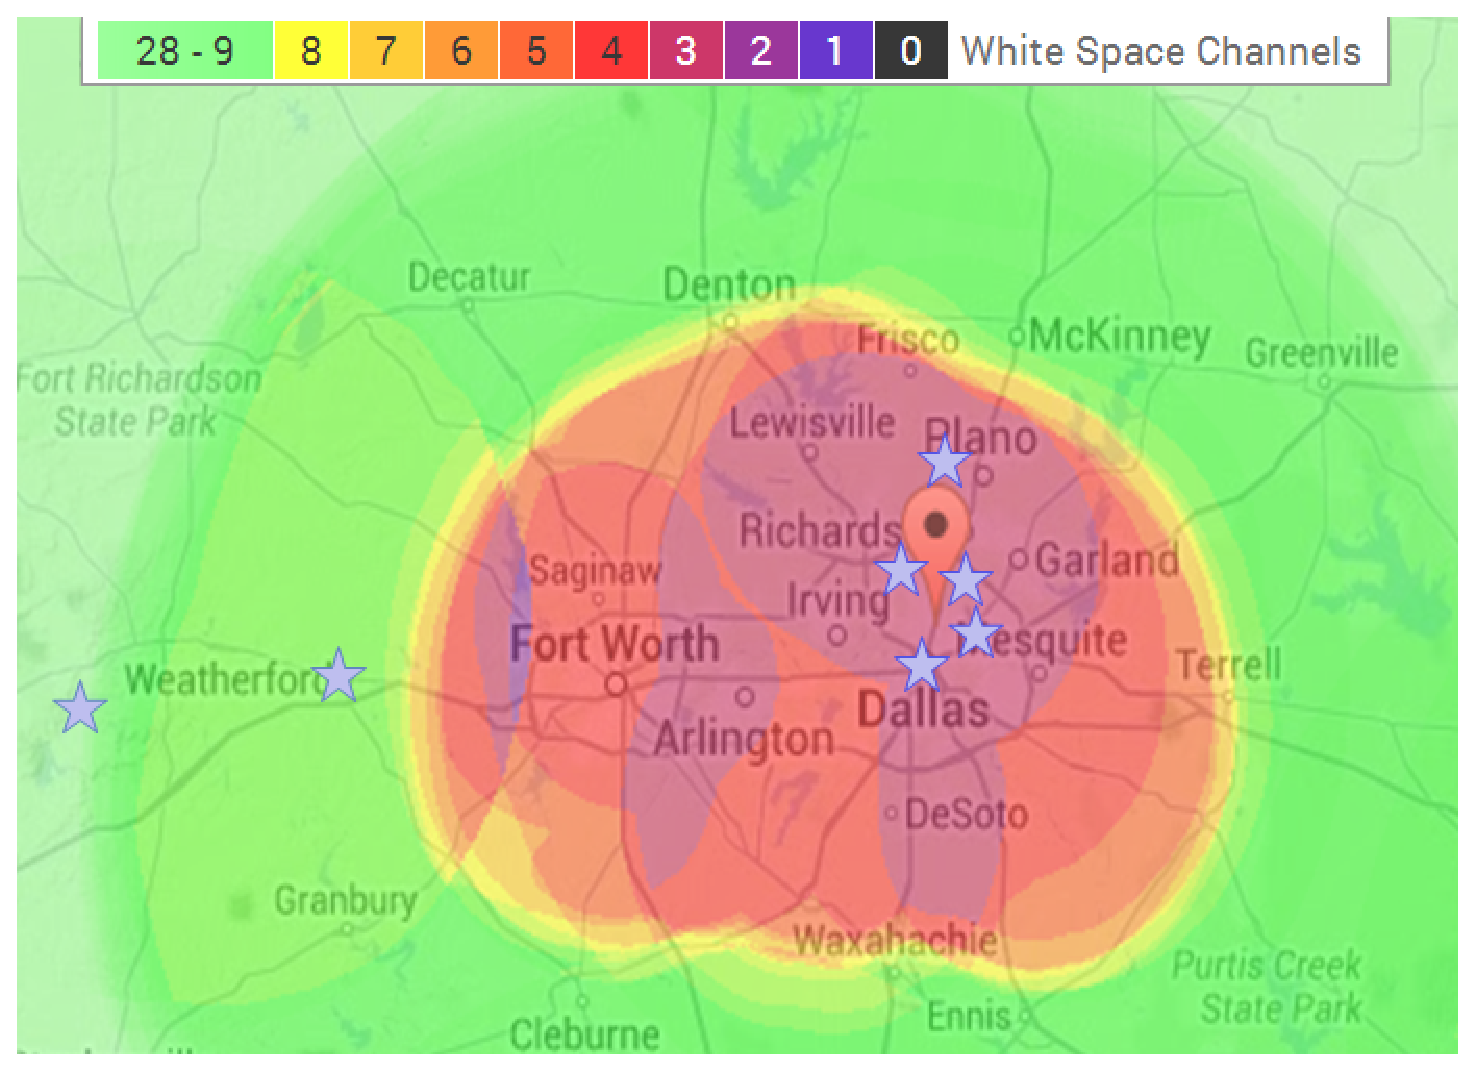
\includegraphics[width=74mm]{figures/drivemap}
\vspace{-0.1in}
\caption{White Space Channels in DFW Metropolitan and Surrounding Areas.}                                                                 
\label{fig:drivemap}
\vspace{-0.1in}
\end{figure}
   
\begin{figure}
%\vspace{-0.0in}
\centering
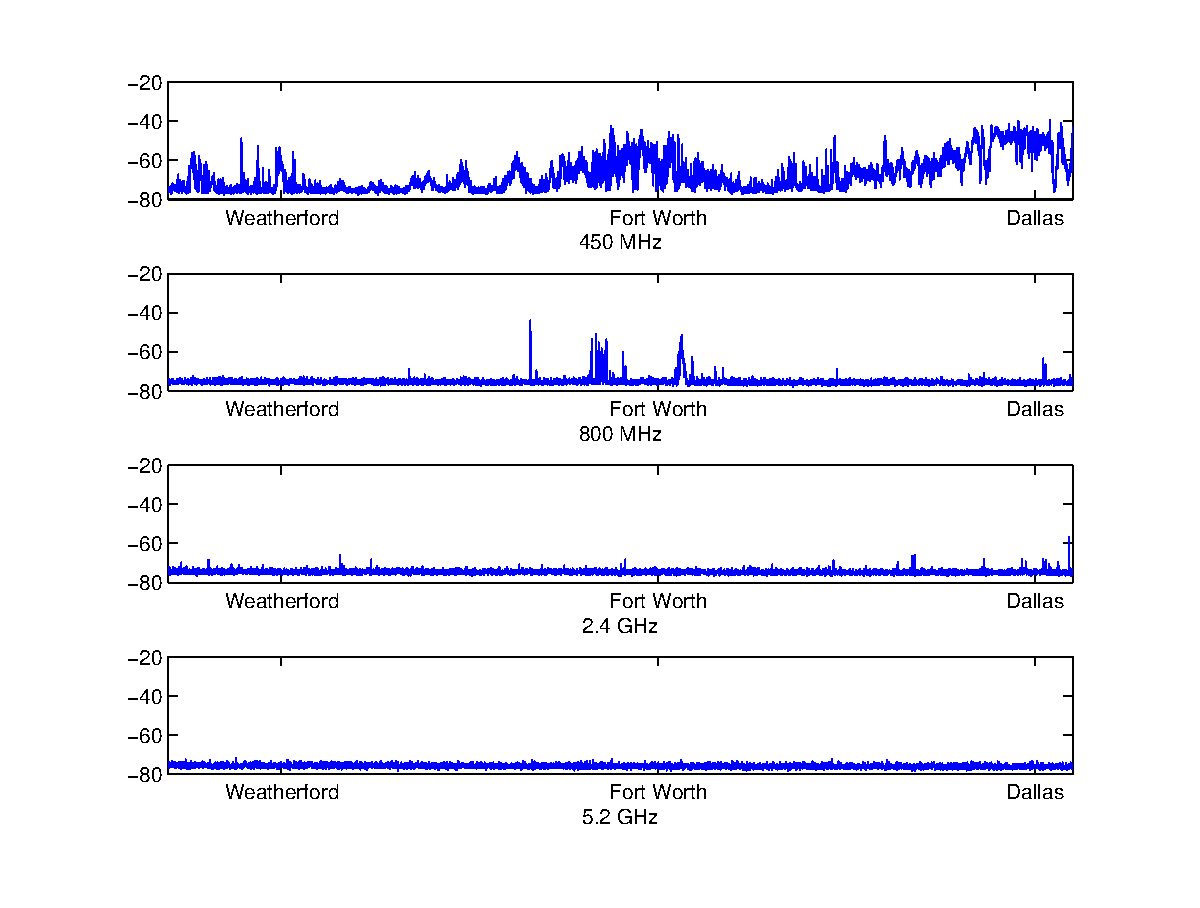
\includegraphics[width=94mm]{figures/drivetest}
\vspace{-0.4in}
\caption{Spectrum Activity in DFW Metropolitan and Surrounding Areas.}                                                                 
\label{fig:drivetest}
\vspace{-0.3in}
\end{figure}




% Here

The activity level calculated with our measurements are shown in Table~\ref{tab:activitymeasurement}. Dallas, the 
city with the greatest population in North Texas, has the highest activity level in most of the measured bands, 
especially at 450 MHz. The Dallas urban measurements are taken from the SMU campus, two neighborhoods, and a 
densely-populated suburb (Plano). Our measurements indicate that 2.4 GHz has a higher activity level in urban area 
than the measured downtown area. Most schools and their neighborhoods are covered by WiFi, which contributes to the 
high activity level at 2.4 GHz and 5.2 GHz. In Weatherford, all the bands have lower activity levels than in Dallas. 
A peculiarity in the measurements can be seen by the sparse area in Weatherford having more activity than the other 
regions for 450 MHz. This can be explained due to the measurement location being on the East of Weatherford (closer 
to Fort Worth, which has a population of approximately 750k). Millsap is a typical sparse rural area with approximately 
500 total residents. The activity levels across all the bands are lower than in Dallas and Weatherford. In the 450 MHz 
band, the activity level decreases much faster than in other bands in Dallas and Weatherford. 

\begin{table*}
\centering % centering table 
\begin{tabular}{|l|c|c|c|c|c|c|c|c|c|c|c|} % creating 12 columns 
\hline %\hline % inserting double-line 
Bands     & \multicolumn{3}{c|}{Dallas} & \multicolumn{3}{c|}{Weatherford} & \multicolumn{3}{c|}{Millsap} \\% [0.5ex]
\hline % inserts single-line 
% Entering 1st row 
Area Type & Downtown & Residential & Suburban & Downtown &  Residential & Sparse & Downtown & Residential & Sparse \\ % [0.5ex]
\hline % inserts single-line 
450 MHz &24.37	&25.83  &23.77	&6.05 &12.50  &14.03 & 7.00 & 0.07 & 0.02 \\      
\hline % inserts single-line                                                                                                       
800 MHz &4.40 	&16.49  &4.77	&5.22&5.07 &4.43  & 3.87 & 4.20 & 3.60 \\      
\hline % inserts single-line                                                                                                      
2.4 GHz &15.87 	&34.95  &2.60	&2.03&2.03 &2.77  & 2.07 & 1.60 & 0.80 \\      
\hline % inserts single-line                                                                                                     
5.2 GHz &19.70	&35.46  &1.53	&1.93&1.93 &1.33  & 1.27 & 2.07 & 2.10 \\      
\hline % inserts single-line 
\end{tabular}    
\caption{Activity Level in Multiple Locations} % title name of the table 
\label{tab:activitymeasurement}    
\vspace{-0.3in}
\end{table*}    


% Need a summary
Our measurements verify the channel occupation variation in DFW metroplex and quantify the occupation
through measurements based activity level. The results induce the spectrum bands are higher occupied in
dense populated areas than sparse areas with different levels of utility across bands. The measurements 
methods and quantification provides the way to get the knowledge of the target environment. We apply these 
measurements to our MAPE framework\ref{sec:winmee} and BPS algorithms\ref{sec:whitemesh} to further solve the 
access tier network deployment and multiband channel assignments.
